% !TEX root = talk.tex
\section[Introduction]{What are \TeX, \LaTeX\ and Friends?}
\begin{frame}
\frametitle{What are \TeX\ and \LaTeX,\ and Friends?}

\begin{description}
\item<1>[\TeX] 
\begin{itemize}
\item \textsmaller{ASCII} \texttt{TeX}, \textsmaller{\textipa{/tEx/}, \textipa{/tEk/}}
\item A \structure{computer typesetting system} created by Donald Knuth
\item for `the creation of beautiful books'
\end{itemize}


\item<2>[\LaTeX]
\begin{itemize}
\item \textsmaller{ASCII} \texttt{LaTeX}, \textsmaller{\textipa{/"leItEx/}, \textipa{/"leItEk/}, \textipa{/"lA:tEx/}, \textipa{/"lA:tEk/}}
\item A \structure{document preparation system} by Leslie Lamport
	\end{itemize}

\pause

\item<3-4>[Binaries]
	\begin{itemize}
  \item \structure{\hologo{eTeX}}: additional primitives to \hologo{TeX}
	\item \structure{\alert<4>{\hologo{pdfTeX}}}: additional PDF-related primitives
  \item \structure{\XeTeX}: native UTF-8 input; can access system fonts
	\item \structure{\hologo{LuaTeX}}: includes the Lua scripting engine
\end{itemize}
\item <5>[Friends]
\begin{itemize}
\item \structure{\BibTeX}, \structure{\MakeIndex}, \structure{\METAFONT}, \structure{METAPOST},  \ldots
\item \url{http://www.ctan.org/what_is_tex.html}
\end{itemize}
\end{description}
\end{frame}

\begin{frame}
\frametitle{Why?}
\framesubtitle{From \url{http://www.ctan.org/what_is_tex.html}}
\begin{columns}[T]
\begin{column}{.46\textwidth}
\begin{block}{Output Quality}
\begin{itemize}
\item It has the best output.
\item It knows typesetting.
\end{itemize}
\end{block}

\begin{block}{Superior Engineering}
\begin{itemize}
\item It's fast.
\item It's stable.
\item It's not rigid (extensible).
\item Plain text input.
\item Many output types.
\end{itemize}
\end{block}
\end{column}

\begin{column}{.46\textwidth}
\begin{block}{Freedom}
\begin{itemize}
\item It's free.
\item It runs anywhere.
\end{itemize}
\end{block}

\begin{block}{Popularity}
\begin{itemize}
\item It's the standard (in academia and science).
\end{itemize}
\end{block}
\end{column}
\end{columns}
\end{frame}

\begin{frame}
\frametitle{Where Would I Want to Use \hologo{LaTeX}?}
\begin{itemize}
\item Documents with complex structures
\item Lots of mathematics \pause(or other specific needs)\pause
\item When publishers \alert{require} them
\pause
\item Batch processing
\pause
\item Back-end of other applications
\end{itemize}
\end{frame}

\begin{frame}
\frametitle{How Do I Use It?}
\begin{enumerate}
\item<+-> Write a plain text \hologo{LaTeX} file (\texttt{.tex})
\item<+-> Run it through \texttt{pdflatex} or \texttt{xelatex} $\rightarrow$ \textsmaller{PDF} output\\
\textsmaller{(or \texttt{latex + dvips + ps2pdf} for \textsmaller{DVI} + \textsmaller{PS} + \textsmaller{PDF})}
\item<+-> Run \texttt{bibtex} and/or \texttt{makeindex} to process bibliographies, indices
\item<+-> Re-run \texttt{pdflatex} to resolve references and pointers
\end{enumerate}
\end{frame}

\begin{frame}[fragile]
\frametitle{Example \texttt{.tex} File}

\begin{columns}[T]
\begin{column}{.47\textwidth}
\begin{beamerboxesrounded}[width=\linewidth]{}
\vskip-1.2em
\begin{lstlisting}[moretexcs={maketitle,tableofcontents,subsection},
emph={document,abstract},
basicstyle={\ttfamily\footnotesize\lsstyle},lineskip=-2pt]
\documentclass[a4paper,11pt]{article}
\author{Lim Lian Tze}
\title{An Introductory Paper}
\date{\today}
:\onslide<1-3>{{\bfseries\color{Maroon}\textbackslash usepackage}[\textcolor{Sienna2}{\bfseries english}]\{\textcolor{RoyalBlue3}{\bfseries babel}\}}%
\onslide<4|trans:0|handout:0>{\llap{{\bfseries\color{Maroon}\textbackslash usepackage}[\textcolor{Sienna2}{\bfseries ngerman}]\{\textcolor{RoyalBlue3}{\bfseries babel}\}}}%
\onslide<5|trans:0|handout:0>{\llap{{\bfseries\color{Maroon}\textbackslash usepackage}[\textcolor{Sienna2}{\bfseries bahasam}]\{\textcolor{RoyalBlue3}{\bfseries babel}\}}}:

\begin{document}
\maketitle
\tableofcontents

\begin{abstract}
This paper introduces\ldots
\end{abstract}

\section{Introduction}
We consider\ldots

\section{State of the Art}
We look at\ldots

\subsection{Document Formats}
There are many\ldots
\end{document}
\end{lstlisting}
\vspace*{-1.2em}
\end{beamerboxesrounded}
\end{column}

\begin{column}{.46\textwidth}
\hfill\uncover<3>{\fcolorbox{black}{white}{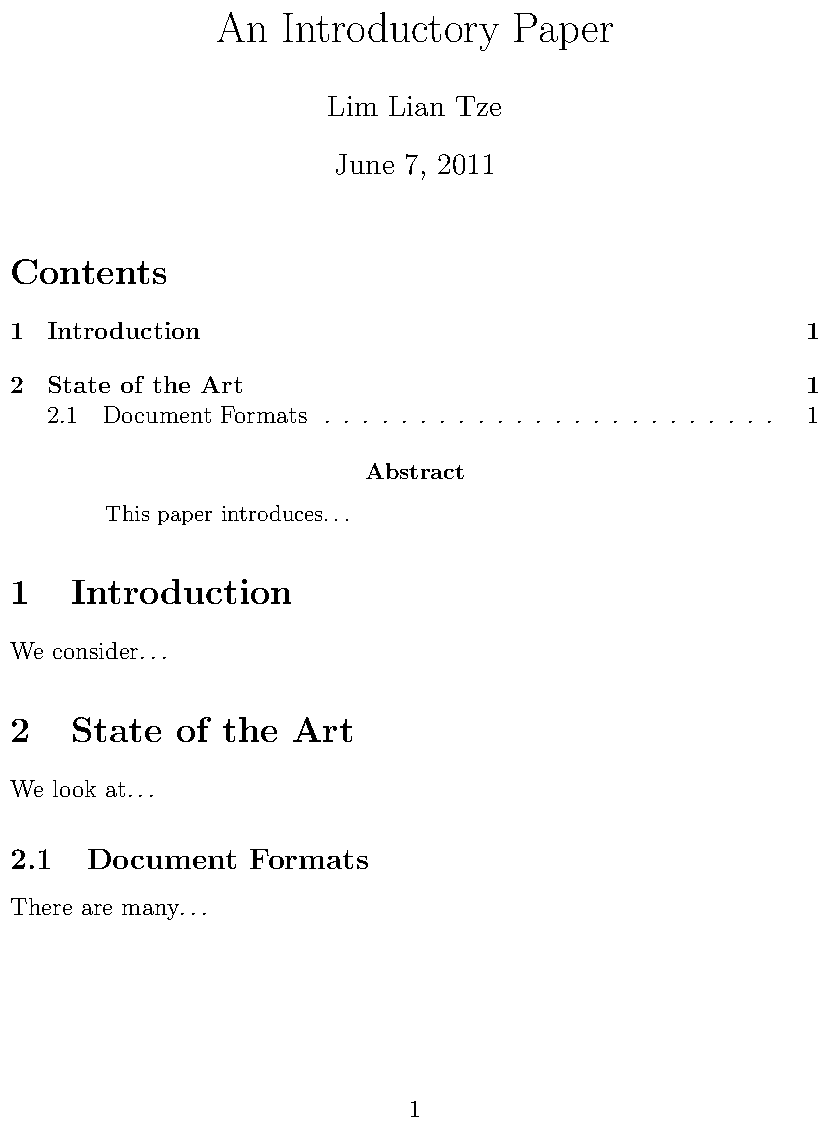
\includegraphics[width=.95\linewidth]{examples/first-en}}}%
\uncover<4|trans:0|handout:0>{\llap{\fcolorbox{black}{white}{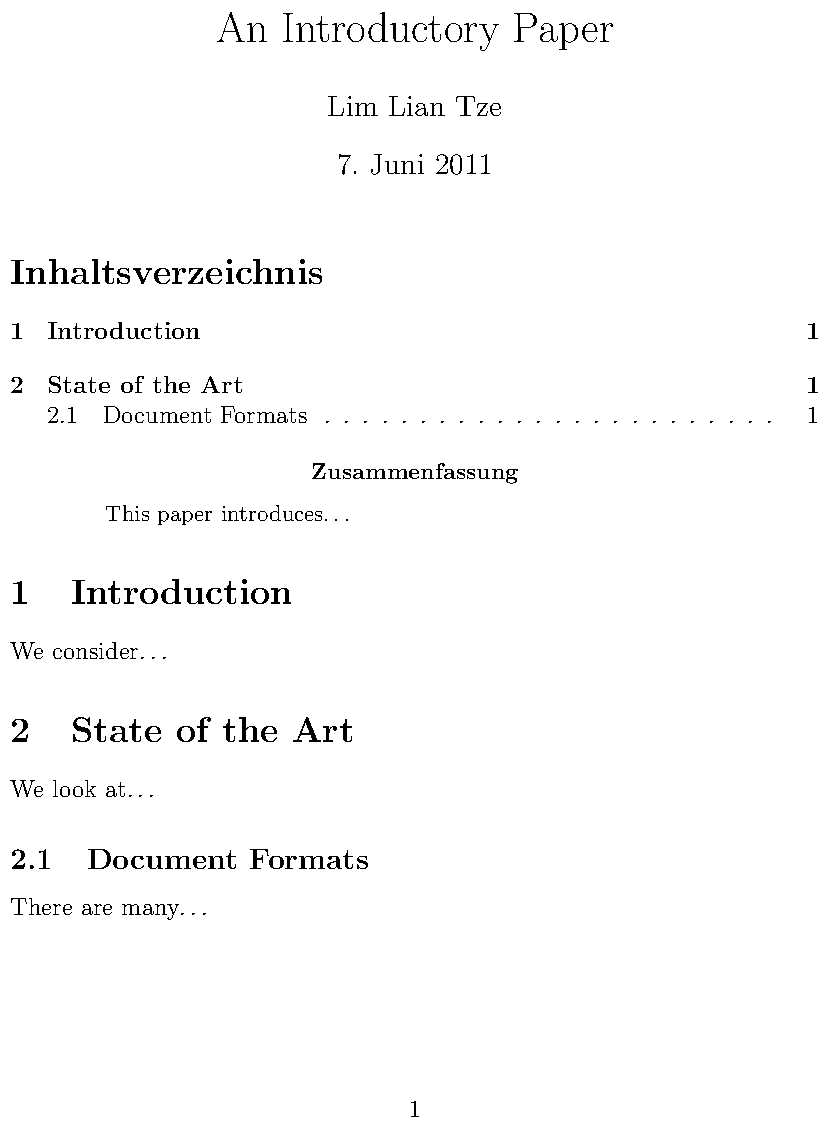
\includegraphics[width=.95\linewidth]{examples/first-de}}}}%
\uncover<5|trans:0|handout:0>{\llap{\fcolorbox{black}{white}{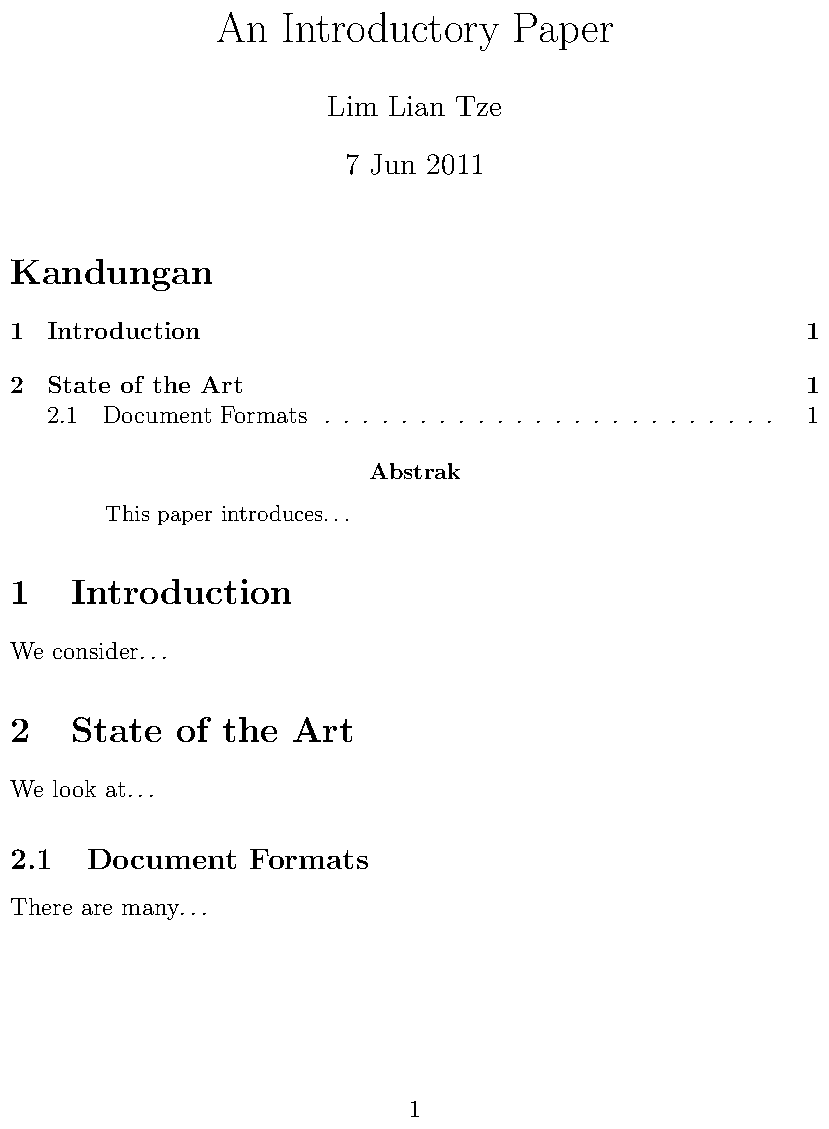
\includegraphics[width=.95\linewidth]{examples/first-ms}}}}
\end{column}
\end{columns}

\uncover<2->{\tikz[remember picture,overlay]\node[single arrow,fill=DarkSeaGreen,font=\ttfamily\bfseries,xshift=-1em] at (current page.center) {pdflatex};}

\end{frame}

\begin{frame}
\frametitle{Where Do I Get It?}
\begin{description}
\setlength\labelwidth{8.5em}
\setlength\itemindent{3em}
\item[Windows] \MikTeX, \TeX Live
\item[Un*x, \textsmaller{GNU}/Linux] \TeX Live
\item[Mac OS X] Mac\TeX\ (based on \TeX Live)
\item[Installation] Use your OS' package manager\\\hspace{\itemindent}(or download manually)
\pause
\item[Editors] vi, emacs, Texmaker, TeXworks, \ldots
\pause
\item[\hologo{LaTeX} Packages] Use \MikTeX\ or \TeX Live's package manager
\pause
\item[Documentation] 
{\small (\TeX Live)} \texttt{\$ texdoc <package name>}\\
\hspace{\itemindent}{\small (\MikTeX)} \texttt{\$ mthelp <package name>}
\end{description}
\end{frame}

\begin{frame}
\frametitle{Easy to Learn, Hard to Master}
\begin{itemize}
\item<+-> Customising may not be straightforward (vs word processors)
\item<+-> Intentionally so: Style guidelines should be followed strictly
\begin{itemize}
\item Publisher/organisation provides \structure{\texttt{document class}} or \structure{\texttt{style}} files
\item Use these to take care of formatting and styling, focus on the \structure{content}
\end{itemize}
\item<+-> Fair enough. \\But where do I learn all the stuff the \TeX nicians and \TeX perts do?
\item<+-> (There \emph{is} a learning curve)
\end{itemize}
\end{frame}

\begin{frame}[label=help]
\frametitle{Getting Help}
\begin{itemize}
\item<+-> Many free tutorials and e-books on the Web (beware of obsolete ones!)
\begin{itemize}
\item \structure{Getting to Grips with \hologo{LaTeX}.}\; Andy Roberts. \url{http://www.andy-roberts.net/misc/latex/}
\item \structure{\hologo{LaTeX}: Beautiful Typesetting.}\; Lim Lian Tze. \url{http://liantze.penguinattack.org/latextypesetting.html}
\item \structure{\hologo{LaTeX} and Friends.}\; M.R.C.\ van Dongen. \url{http://csweb.ucc.ie/~dongen/LaTeX-and-Friends.pdf}
\item \structure{The \hologo{LaTeX} WikiBook.}\; \url{http://en.wikibooks.org/wiki/LaTeX}
\end{itemize}

\item<+-> Questions?
\begin{itemize}
\item \hologo{TeX} \textsmaller{FAQ}.\;  \url{http://www.tex.ac.uk/cgi-bin/texfaq2html}
\item \hologo{TeX}.SX.\; \url{http://tex.stackexchange.com/}
\item \texttt{comp.text.tex} usenet group
\item Malaysian \hologo{LaTeX} User Group.\; \url{http://latex-my.blogspot.com/}
\end{itemize}

\item<3-> Arrange for training
\end{itemize}
\end{frame}


\begin{frame}
\centering\Huge
So, What Can \hologo{LaTeX} Do?
\par
\end{frame}